\documentclass{article}

\usepackage{graphicx}
\usepackage{tikz}
\usepackage{tikzsymbols}
\usetikzlibrary{calc,patterns,shapes.geometric}
\pagestyle{empty}
\usepackage[margin=0pt]{geometry}
\geometry{papersize={14in,12in}}

\def\centerarc[#1](#2)(#3:#4:#5){\draw[#1] ($(#2)+({#5*cos(#3)},{#5*sin(#3)})$) arc (#3:#4:#5);}

\begin{document}
	\begin{figure}
		\centering
		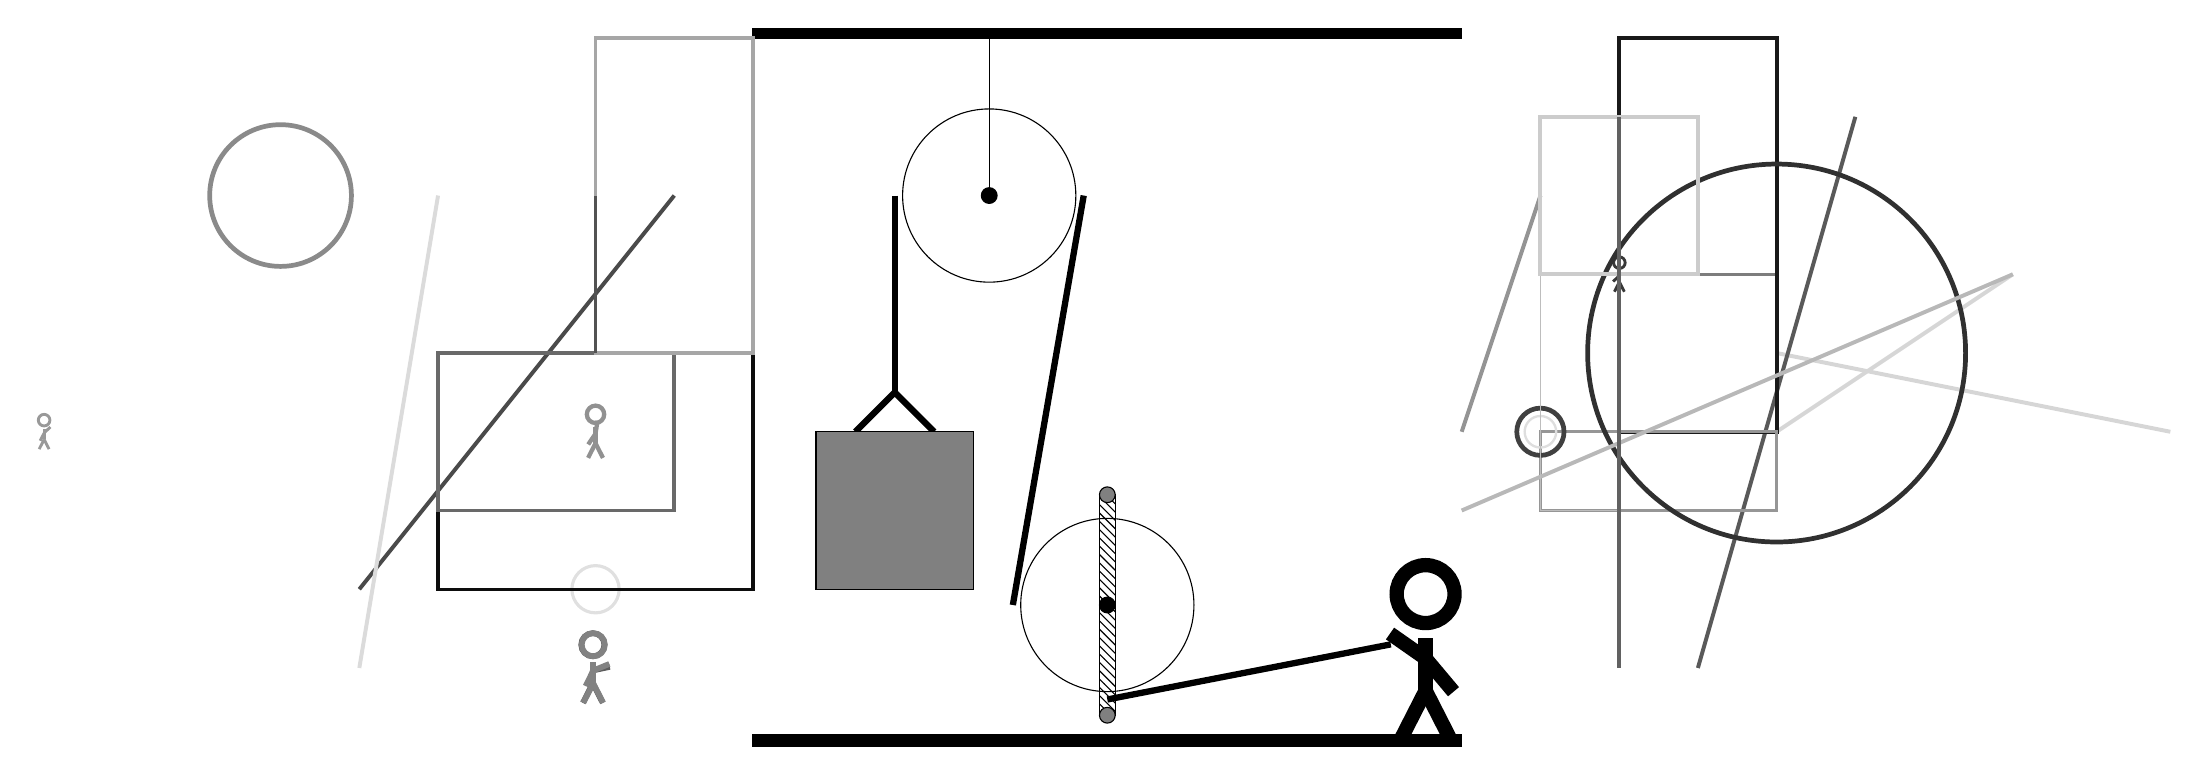
\begin{tikzpicture}
			%%%%% START %%%%%
			
			\draw[fill=black] (-2, 9) rectangle (7, 9.125);
			
			\draw (1, 7) circle (1.1);
			\draw[fill=black] (1, 7) circle (0.1);
			\draw (1, 9) -- (1, 7);
			
			\draw[line width=0.4mm, color=black!51] (9, 4) rectangle (11, 6);
			
			\node[line width=0.3mm, color=black!78] at (9, 6) {\Strichmaxerl[2][44][90]};
			\draw[line width=0.5mm, color=black!16](11, 5) -- (16, 4);
			\draw[line width=0.5mm, color=black!42](7, 4) -- (8, 7);
			
			\node[line width=0.7mm, color=black!40] at (-11, 4) {\Strichmaxerl[2][63][44]};
			\draw [line width=0.4mm, color=black!12](-4, 2) circle (0.3);
			\draw[line width=0.5mm, color=black!71](-7, 2) -- (-3, 7);
			\node[line width=0.7mm, color=black!64] at (-4, 1) {\Strichmaxerl[4][88][12]};
			\draw[line width=0.5mm, color=black!16](11, 4) -- (14, 6);
			\draw[line width=0.5mm, color=black!65](12, 8) -- (10, 1);
			\draw[line width=0.5mm, color=black!90] (9, 4) rectangle (11, 9);
			\draw[line width=0.4mm, color=black!41] (8, 4) rectangle (11, 3);
			\draw [line width=0.6mm, color=black!81](11, 5) circle (2.4);
			
			\draw [line width=0.3mm, color=black!13](8, 4) circle (0.2);
			\draw[line width=0.5mm, color=black!14](-6, 7) -- (-7, 1);
			\draw[line width=0.5mm, color=black!28](7, 3) -- (14, 6);
			
			\draw[line width=0.4mm, color=black!95] (-2, 5) rectangle (-6, 2);
			\draw [line width=0.6mm, color=black!75](8, 4) circle (0.3);
			\draw[line width=0.5mm, color=black!59] (-3, 3) rectangle (-6, 5);
			\draw[line width=0.4mm, color=black!35] (-2, 5) rectangle (-4, 9);
			\draw[line width=0.5mm, color=black!68](-4, 5) -- (-4, 7);
			
			\draw[line width=0.2mm, color=black!26] (9, 6) rectangle (8, 3);
			\node[line width=0.3mm, color=black!43] at (-4, 4) {\Strichmaxerl[3][56][81]};
			\draw[line width=0.5mm, color=black!20] (8, 6) rectangle (10, 8);
			\node[line width=0.2mm, color=black!49] at (-4, 1) {\Strichmaxerl[4][64][22]};
			
			\draw[line width=0.5mm, color=black!62](9, 1) -- (9, 8);
			
			\draw [line width=0.6mm, color=black!46](-8, 7) circle (0.9);
			
			\draw[fill=white](2.5, 1.8) circle (1.1);
			\draw[fill=black] (2.5, 1.8) circle (0.1);
			\draw[pattern=north west lines, pattern color=black] (2.4, 3.2) rectangle (2.6, 0.4);
			\draw[fill=black!50] (2.5, 3.2) circle (0.1);
			\draw[fill=black!50] (2.5, 0.4) circle (0.1);
			
			\draw[line width=0.8mm] (-0.7, 4.0) -- (-0.2, 4.5) -- (0.3, 4.0);
			\draw[fill=black!50] (-1.2, 4.0) rectangle (0.8, 2.0);
			
			\draw[line width=0.8mm] (-0.2, 7) -- (-0.2, 4.5);
			\centerarc[line width=0.8mm](1, 7)(0:180:1.2000000000000002);
			\draw[line width=0.8mm](2.2, 7) -- (1.3, 1.8);
			\centerarc[line width=0.8mm](2.5, 1.8)(180:270:1.2000000000000002);
			\draw[line width=0.8mm](2.5, 0.6) -- (6.1, 1.3);
			
			\node at (6.5, 1.2) {\Strichmaxerl[10][-35][-50]};
			
			\draw[fill=black] (-2, 0) rectangle (7, 0.15);
			
			%%%%% END %%%%%
		\end{tikzpicture}
	\end{figure}	
\end{document}